\documentclass[border=4pt]{standalone}
% Shared by the independently buildable vector figures.
\usepackage[T1]{fontenc}
\usepackage{amsmath,amssymb,newpxtext,newpxmath}
\usepackage[semibold]{sourcesans}
\usepackage{pgfplots}
\pgfplotsset{compat=1.18}
\usetikzlibrary{arrows.meta,calc,positioning}
\usepgfplotslibrary{groupplots}
\definecolor{ink}{HTML}{19303A}
\definecolor{sea}{HTML}{00675E}
\definecolor{clay}{HTML}{A24725}
\definecolor{muted}{HTML}{4C636C}
\definecolor{rulegray}{HTML}{CAD4D4}
\definecolor{wash}{HTML}{EAF4F0}
\definecolor{warm}{HTML}{F7EEE5}
\color{ink}
\tikzset{every picture/.style={font=\sffamily\small},
  arrow/.style={-{Stealth[length=2mm]},line width=.8pt,draw=muted}}
\pgfplotsset{companion/.style={axis lines=left,axis line style={draw=muted},
  tick style={draw=muted},ticklabel style={font=\sffamily\footnotesize,text=muted},
  label style={font=\sffamily\small},grid=major,grid style={draw=rulegray!64,line width=.25pt},
  tick align=outside,enlarge x limits=false,scaled ticks=false,
  every axis plot/.append style={line join=round},
  legend style={draw=none,fill=none,font=\sffamily\footnotesize},
  title style={font=\sffamily\bfseries\small,anchor=south west,at={(0,1.03)}}}}

\begin{document}
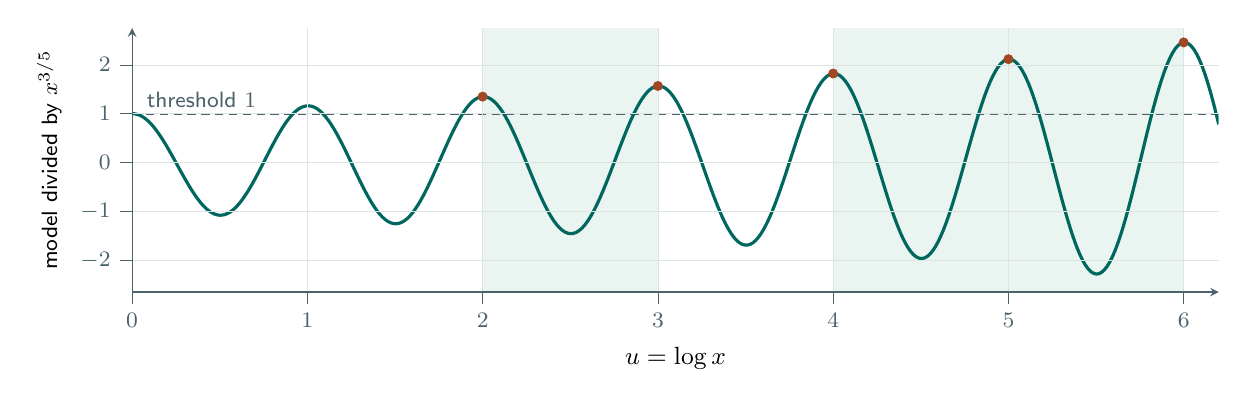
\begin{tikzpicture}
\begin{axis}[companion,axis on top,width=13.8cm,height=3.35cm,scale only axis,xmin=0,xmax=6.2,
  ymin=-2.65,ymax=2.75,xtick={0,1,2,3,4,5,6},ytick={-2,-1,0,1,2},
  xlabel={$u=\log x$},ylabel={model divided by $x^{3/5}$},ylabel style={font=\sffamily\footnotesize}]
\path[fill=wash] (axis cs:2,-2.65) rectangle (axis cs:3,2.75);
\path[fill=wash] (axis cs:4,-2.65) rectangle (axis cs:6,2.75);
\addplot[muted,densely dashed,line width=.8pt] coordinates {(0,1) (6.2,1)};
\addplot[sea,line width=1.15pt,domain=0:6.2,samples=400] {exp(.15*x)*cos(360*x)};
\addplot[only marks,mark=*,mark size=1.6pt,clay,domain=2:6,samples=5] {exp(.15*x)};
\node[anchor=south west,font=\sffamily\footnotesize,text=muted,fill=white,inner sep=1.3pt]
  at (axis cs:.06,1.05){threshold $1$};
\end{axis}
\end{tikzpicture}
\end{document}
